% Settings for the default beamer theme
\documentclass[english, aspectratio=169]{beamer}
\usepackage[T1]{fontenc}
\usepackage[utf8]{inputenc}
\usepackage{tabularx}
\usepackage{babel}
\usepackage[ruled,vlined]{algorithm2e}
\SetAlgorithmName{Algoritmus}{algoritmus}{List of Algorithms}
\setcounter{secnumdepth}{3}
\setcounter{tocdepth}{3}

\makeatletter

\newcommand\makebeamertitle{\frame{\maketitle}}

% (ERT) argument for the TOC
\AtBeginDocument{%
  \let\origtableofcontents=\tableofcontents
  \def\tableofcontents{\@ifnextchar[{\origtableofcontents}{\gobbletableofcontents}}
  \def\gobbletableofcontents#1{\origtableofcontents}
}

% Theme settings
\usetheme{Frankfurt}
\usecolortheme{default}
\usefonttheme[onlymath]{serif}

% Template settings
\setbeamertemplate{navigation symbols}{}
\setbeamertemplate{blocks}[rounded][shadow=false]
\setbeamertemplate{title page}[default][colsep=-4bp, rounded=true, shadow=false]
\makeatother

\begin{document}

% Title page
\section{Ismétlés}
\title[]{Üzleti Intelligencia}
\subtitle{4. Előadás: Monte Carlo és temporális különbségek}
\author[Kuknyó Dániel]{Kuknyó Dániel\\Budapesti Gazdasági Egyetem}
\date{2023/24\\1.félév}
\makebeamertitle

% Table of contents slide
\begin{frame}
\tableofcontents{}
\end{frame}

% Table of contents of the current section
\begin{frame}
\tableofcontents[currentsection]
\end{frame}

\begin{frame}{Az RL modellje}
\begin{columns}
\begin{column}{.5\textwidth}
\only<1>{\begin{block}{Markov döntési folyamat}
\[
MDP\left(S,A,P,R,s_{0},\gamma\right)
\]
\begin{itemize}
	\item $S$: állapotok halmaza
	\item $A$: cselekvések halmaza
	\item $P:\; S \times A \times S \rightarrow [0,1]$: állapotátmeneti valószínűségek
	\item $R:\; S \times A \rightarrow \mathbb{R}$: azonnali jutalmak
	\item $s_{0}$: kezdőállapot
	\item $\gamma$: diszkont faktor
\end{itemize}
\end{block}}
\only<2>{Az MDP folyamata:\\
\begin{enumerate}
	\item Az ügynök $s_{0}$ állapotból indul
	\item Az ügynök $\pi$ politika szerint cselekszik: $a_{t}\sim\pi(s_{t})$
	\item A környezet reagál a cselekvésre, és visszaadja az ügynöknek $r_{t+1}$ jutalmat és $s_{t+1}$ következő állapotot
	\item Ez ismétlődik amíg a kilépési kritérium be nem teljesül
\end{enumerate}
Cél: Az optimális politika megtalálása. A politika optimális, ha a hozamának várható értéke maximális:
\[
E_{\pi}\left(r_{1} + \gamma r_{2} + \gamma^{2}r_{3} + ...\right) \rightarrow max
\]}
\end{column}
\begin{column}{.5\textwidth}
\begin{center}
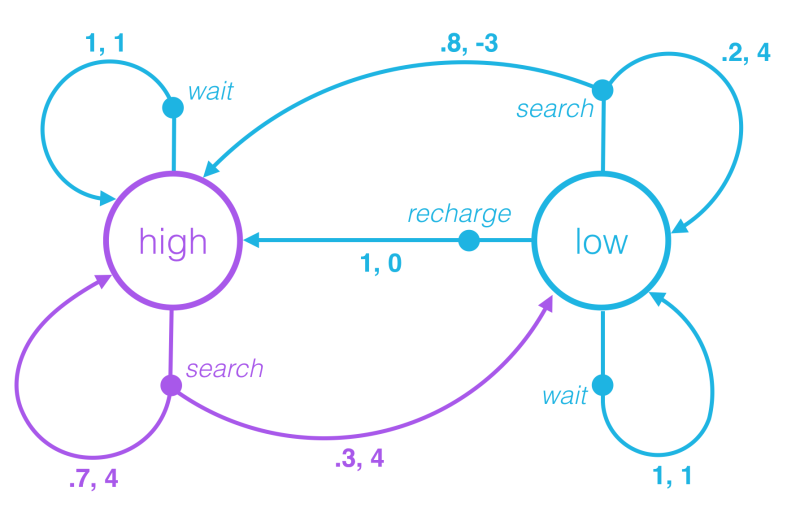
\includegraphics[width=7cm, height=7cm, keepaspectratio]{images/mc_td_1.png}
\end{center}
\end{column}
\end{columns}
\end{frame}

\section{Monte Carlo}

\begin{frame}{Monte Carlo becslés}
\begin{columns}
\begin{column}{.6\textwidth}
\only<1>{A dinamikus programozási algoritmusok futtatásához szükség volt a környezet dinamikájának modelljére. Ez a tulajdonságuk gyakran használhatatlanná teszik őket a gyakorlatban, mert a környezeti dinamika vagy nem ismert vagy nem kiszámítható sok esetben. \par\smallskip
A Monte Carlo (\textbf{MC}) módszerek ezzel szemben nem igényelnek előzetes tudást a feladat elvégzéséhez: csak \textbf{tapasztalat} szükséges ahhoz, hogy megtanuljanak elvégezni egy feladatot. Ezt úgy érik el, hogy mintát vesznek állapotokból, cselekvésekből és jutalmakból, majd az eredményeket átlgolják.}
\only<2>{\begin{center}
\begin{block}{Monte Carlo szimuláció}
Számítási algoritmusok olyan osztálya, ami a véletlen vagy bizonytalan komponens hatását analizálja vagy szimulálja sztochasztikus folyamatokban. 
\end{block}
\end{center}}
\end{column}
\begin{column}{.4\textwidth}
\begin{center}

\includegraphics[width=6cm, keepaspectratio]{images/mc_td_2.png}
\end{center}
\end{column}
\end{columns}
\end{frame}

\begin{frame}{Monte Carlo a megerősítéses tanulásban}
\begin{columns}
\begin{column}{.5\textwidth}
A MC tanítási algoritmus a politika iteráció egy általánosított változata. A megerősítéses tanulásban a MC algoritmusok a mélységi bejárásnak felelnek meg. \par\smallskip
A MC módszer egy egyszerű ötletet használ: epizódonkénti nyers tapasztalatok alapján tanul anélkül, hogy modellezné a környezeti dinamikát. A megfigyelt átlagos hozamot a várható megtérülésre tett becslésként számítja ki. 
\begin{block}{}
\[
V(s_{t}) \leftarrow V(s_{t}) + \alpha \left[ G_{t} - V(s_{t}) \right]
\]
\end{block}
\end{column}
\begin{column}{.5\textwidth}
\begin{center}
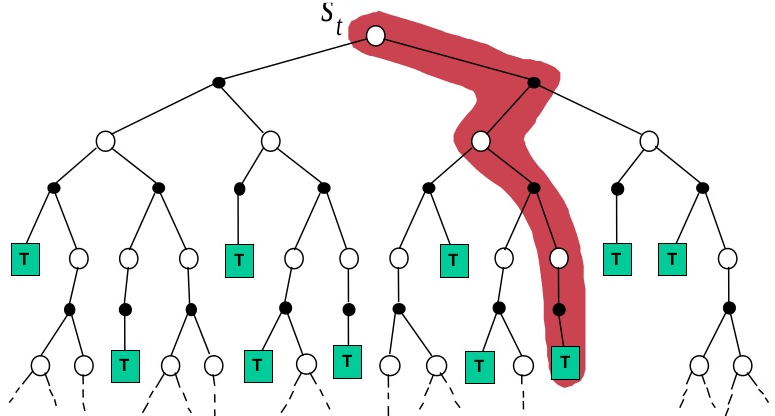
\includegraphics[width=7cm, height=7cm, keepaspectratio]{images/mc_td_3.png}
\end{center}
\end{column}
\end{columns}
\end{frame}

\begin{frame}{Értékfüggvények a Monte Carlo tanításban}
\begin{columns}
\begin{column}{.8\textwidth}
A MC mivel epizódonként vesz mintát a hozamokból az értékfüggvények csak sok epizód hozamának átlagolásaként számítódhatnak ki.\par\smallskip
\only<1>{Az \textbf{állapot-érték függvény} megadja, mennyi a várható hozam, ha az ügynök adott $s$ állapotban áll, és onnan $\pi$ politikát követi:
\begin{block}{}
\[
V_{\pi}(s)=Avg\left\{ G_{t:T}|s_{t}=s \right\}
\]
\end{block}}
\only<2>{Az \textbf{állapot-cselekvés minőség függvény} megadja, mennyi a várható hozam, ha az ügynök adott $s$ állapotban áll, $a$ cselekvést végrehajtja, majd onnan $\pi$ politikát követi:
\begin{block}{}
\[
Q_{\pi}(s,a)=Avg \left\{ G_{t:T} | s_{t}=s, a_{t}=a \right\}
\]
\end{block}}
Ahol
\[
G_{t:T}=\sum_{k=0}^{T-t}\gamma^k r_{t+k}
\]
$t$ aktuális időlépéstől a $T$ terminális állapotba vezető időlépésig az ügynök által összegyűjtött diszkontált kumulált hozam.
\end{column}
\begin{column}{.2\textwidth}
\begin{center}
\only<1>{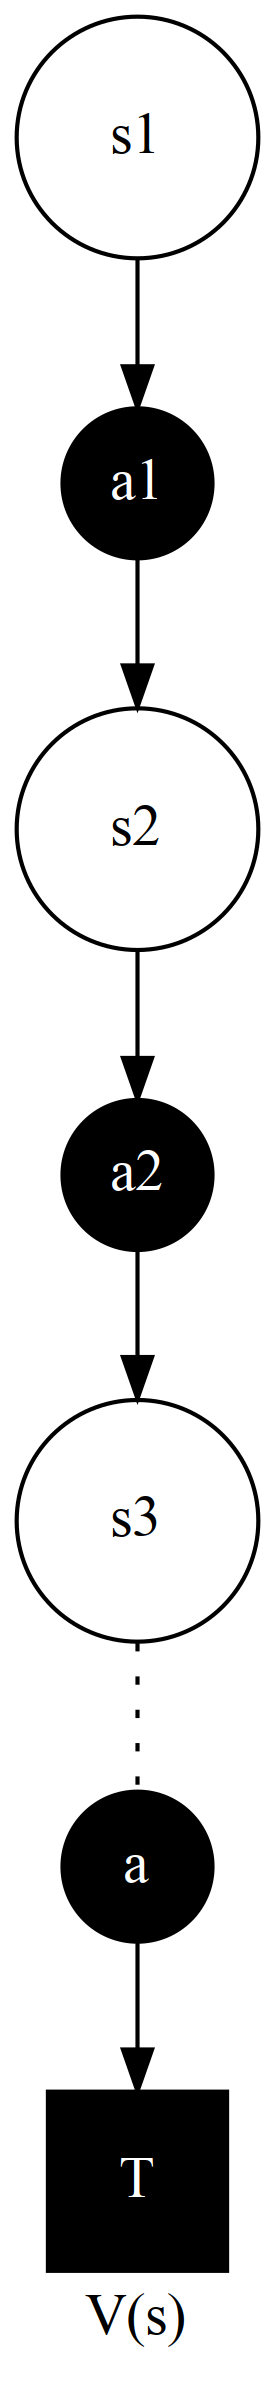
\includegraphics[height=7cm, keepaspectratio]{graphs/mc_td_2.png}}
\only<2>{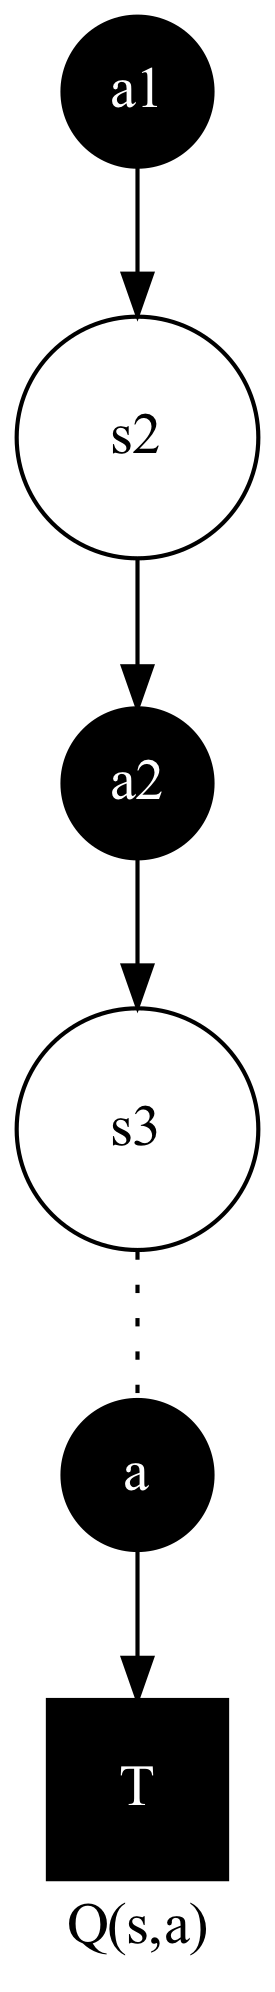
\includegraphics[height=7cm, keepaspectratio]{graphs/mc_td_3.png}}
\end{center}
\end{column}
\end{columns}
\end{frame}


\end{document}





